\documentclass[11pt,a4paper]{article}
\usepackage[top=0.5in, bottom=0.5in,left=1in,right=1in]{geometry} 
\usepackage[utf8]{inputenc}
\usepackage[T1]{fontenc}
\usepackage{mathptmx}
\usepackage{amsfonts}
\usepackage{amsmath, amssymb}
\usepackage{bm}
\usepackage{nccmath}
\usepackage{graphicx}
\usepackage{titling}
\usepackage{indentfirst}
\usepackage{url}
\usepackage{xurl}
\usepackage[backend=biber,style=apa,date=year]{biblatex}
\usepackage{csquotes}
\usepackage{float}
\usepackage{sectsty}
\usepackage{enumitem}
\usepackage{hyphenat}
\usepackage{wrapfig}
\usepackage{hyperref}
\usepackage{enumitem}
\usepackage{titlesec}
\usepackage[skip=0pt]{caption}
\setlength{\parskip}{1em}
\usepackage{tikz}
\usepackage{breakcites}
\usetikzlibrary{positioning}
\usepackage{geometry}
\usepackage{makecell}
 \geometry{
 a4paper,
 left=25.4mm,
 right=25.4mm,
 top=25.4mm,
 bottom=25.4mm
 }
\usepackage{subcaption}
\DeclareMathSymbol{\mh}{\mathord}{operators}{`\-}


\DeclareSourcemap{
  \maps[datatype=bibtex]{
      \map{
        \step[fieldset=urldate, null]
      }
   }
}

\addbibresource{Bio.bib}

%%%%%%%%%%%%%%%%%%%%%%%%%%%%%%%%%%%%%%%%%%%%%%%%%%%%%%%%%%%%%%%%%%%%%%%%%%%%%%%%%%%%%%%%%%%%%%%%%%%%%%%%%%%%

\title{Implementing adaptive operating policies to achieve economic, and groundwater sustainability goals in agriculture using Evolutionary Multi-Objective Direct Policy Search}


\begin{table}[width=.8\linewidth,cols=6,pos=htb!]
\caption{Performance of the selected policies shown in Figure 5}\label{tbl:4}
\begin{tabular*}{\tblwidth}{@{} LLLLLL@{}}
 \toprule
 Solution & O_{avgrev} & O_{avgdepth} & O_{worstrev} & O_{worstdepth\Delta} & O_{rel} \\ 
 \midrule
MaxRev &  13,788 & 100 &  283 & 6.4 & 20\% \\
60\%Rel &  13,222 & 91 & 277 & 5.8 & 60\% \\
MinDepth &  11,141 & 66 & 216 & 5.1 & 100\% \\
\bottomrule
\end{tabular*}
\end{table}

\date{}

\begin{document}

\maketitle

\vspace{-3cm}

\begin{center}
José M. Rodríguez-Flores$^{1,*}$, Rohini S. Gupta $^2$, Harrison B. Zeff $^3$,\\ Patrick M. Reed $^2$, Josué Medellín-Azuara $^1$\\
\end{center}

\begin{center}
\small
$^1$Environmental Systems Program, University of California Merced, CA, USA\\
$^2$Department of Civil and Environmental Engineering, Cornell University, NY, USA\\
$^3$Department of Environmental Sciences and Engineering, University of North Carolina at Chapel Hill, NC, USA\\
$^*$Corresponding Author: jrodriguezflores3@ucmerced.edu
\end{center}


\section*{Abstract}

Increasing irrigation demand has heavily relied on groundwater use, especially in places with highly variable water supplies and vulnerable to drought. Groundwater management in agriculture is becoming increasingly important, as issues from overdraft and groundwater depletion are rising worldwide. However, multiple challenges emerge to implement sustainable groundwater management, such as trade-offs between economic revenues from food production and groundwater sustainability, and uncertainties in the food-water system. In this study we explore the applicability of Evolutionary Multi-Objective Direct Policy Search to find adaptive policies that water agencies and farmers can implement every year such as land use and groundwater use controls and a groundwater pumping fee. Additionally, this method allows policies to respond dynamically as system state conditions change, for example with variable surface water, changing management decisions between wet and dry years. For this study we used the Semitropic Water Storage district located in the San Joaquin Valley, California to provide insight on to ongoing efforts to achieve groundwater sustainability in the state. Our findings demonstrate that adaptive policies can achieve a flexible groundwater management in a wide range of uncertain future scenarios that achieve sustainable objectives. Among these decisions a pumping restriction and reducing inflexible irrigation demand from tree crops are promising alternatives which can support dry-year pumping while maximizing groundwater storage recovery during wet years. Policies suggest that an adaptive pumping fee is the most flexible decision to control pumping and land use. 
 
\section{Introduction}

As irrigation water demand increases due to increased crop acreage and droughts become more frequent, agricultural regions in the world are relying more on groundwater to make up for surface water losses. In Mediterranean climate regions, as California, and arid and semi-arid regions with variable precipitation, groundwater is the primary water source for buffering drought impacts and food security (\cite{malmgren_groundwater_2022,priyan_issues_2021}). Aquifer systems’ flux dynamics are sensitive to changes in temperature, precipitation, and surface water flows, that can be directly impacted by climate change (\cite{cuthbert_global_2019,wu_divergent_2020}). However, the largest impact from climate change is indirectly through changes in land use and water demand by human activities (\cite{taylor_ground_2013}). Globally, groundwater provides 43 percent of the total irrigation needs (\cite{siebert_groundwater_2010}), and such share is expected to increase as surface water scarcity increases (\cite{wada_nonsustainable_2012}). In California, the lack of groundwater management in agriculture have led to stress and depletion of aquifers (\cite{vasco_satellite-based_2019}), affecting dependent ecosystems (\cite{bierkens_non-renewable_2019}), limiting its access to shallow water-table reliant communities (\cite{pauloo_domestic_2020,perrone_dry_2017}), land subsidence (\cite{smith_groundwater_2020}), reduction of groundwater storage and storativity (\cite{alam_post-drought_2021}), degraded water quality (\cite{levy_critical_2021}), among others. 

The largest rate of groundwater depletion in California has been observed in the San Joaquin Valley (SJV) (\cite{ojha_sustained_2018}). The SJV is the most important agricultural region in the United States by economic value (\cite{usda_national_2020}), but also deeply susceptible to drought risk. Most of the region’s snowpack and water supply comes from limited atmospheric-river driven events (\cite{espinoza_global_2018}). Increasing temperatures and evapotranspiration linked to a warming climate are expected to further reduce snowpack runoff and surface water supply (\cite{fernandez-bou_regional_2021,vahmani_will_2022}). Additionally, human factors such as increasing irrigation demand can exacerbate vulnerability and intensity of droughts (\cite{he_intensification_2017}). During the past decade, the agricultural sector has been largely impacted by multi-year droughts (\cite{lund_lessons_2018,medellin-azuara_economic_2022}). Groundwater pumping is used as a buffer to reduce the negative impacts to agricultural production from surface water shortages, but increasing pumping and lack of management have led groundwater to decline reducing the groundwater recovery capacity (\cite{liu_groundwater_2022}).  Additionally, in the SJV there has been an expansion of perennial tree crops, mainly almonds, which is the most important commodity by value in the region (\cite{usda_national_2020}). Although high profitable, the expansion of perennial tree crops represents a less flexible water demand and a higher financial risk to water shortages due to high establishment costs (\cite{mall_water_2019,qin_flexibility_2019}).   

Given the consequences from overdraft in California, the 2014 Sustainable Groundwater Management Act (SGMA) (\cite{dwr_sustainable_2021}) was put in place to require critically over-drafted basins to achieve sustainability in terms of balance in recharge and extraction by 2040. Groundwater Sustainability Agencies (GSAs) are locally formed agencies responsible for developing and enforcing policies to manage water conjunctively to address groundwater sustainability. The state defined guidelines in the Sustainable Management Criteria (\cite{dwr_sustainable_2017}) that GSAs can use to develop management strategies to achieve sustainable goals, including sustainable groundwater levels. The sustainable criteria define a margin of operational flexibility where the groundwater depth can go above the measurable objective but not above the minimum threshold where undesirable results (e.g. dry wells) may occur (Figure 1). With this framework GSAs can develop flexible groundwater management strategies, allowing pumping during dry years and maximizing groundwater recovery during wet years. Furthermore, food production needs to adapt water and land allocation decisions and crop choice, to achieve groundwater sustainability goals and be less vulnerable to surface water shortages. 


 \begin{figure}[H]
    \centering
    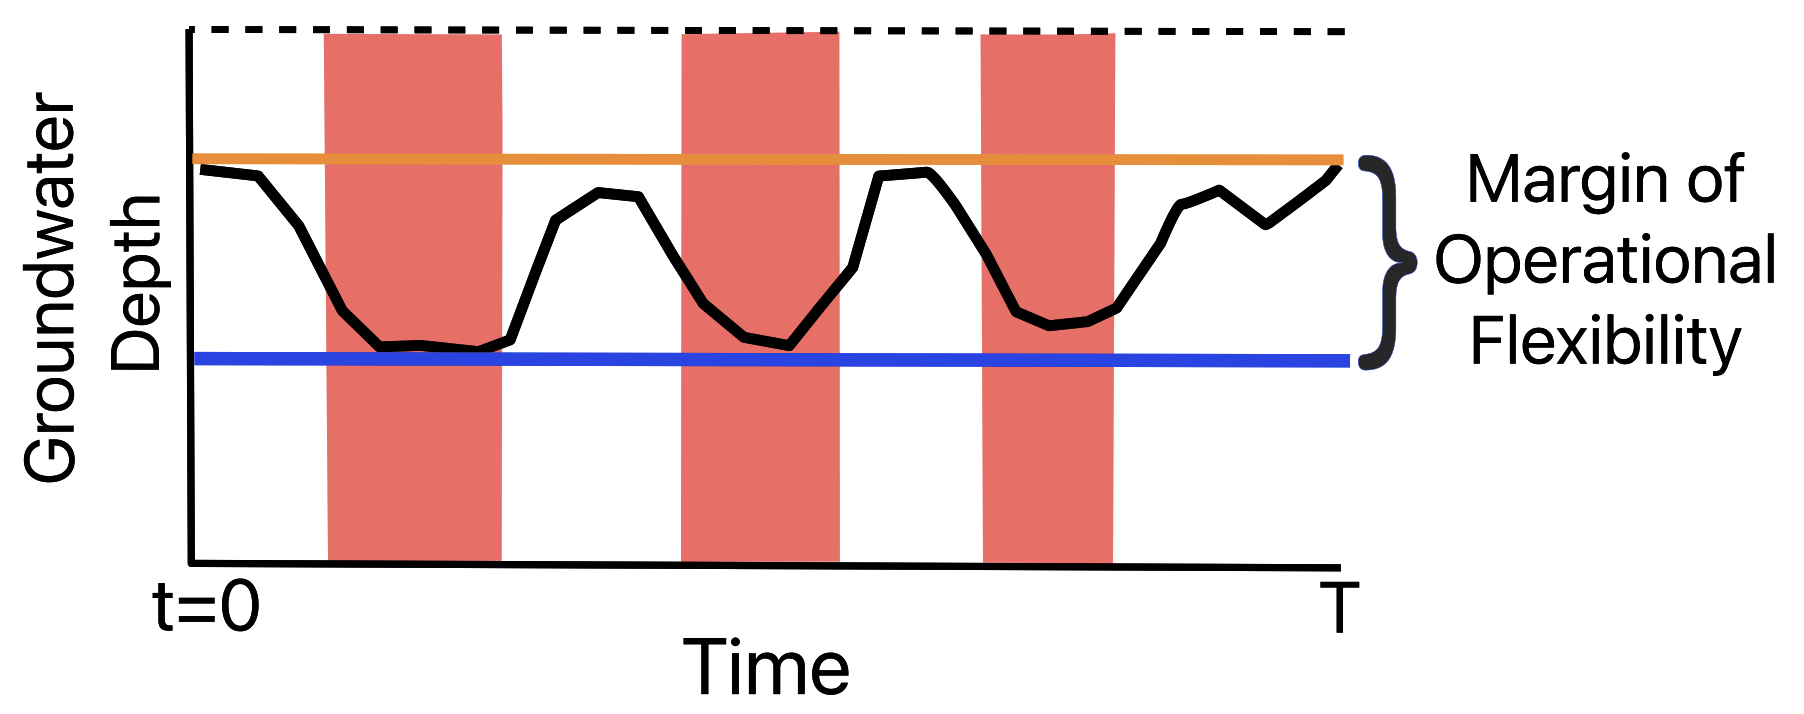
\includegraphics[width=0.7\textwidth]{conceptual_sgma_policy.jpg}
    \caption{Conceptual behavior of groundwater depth under sustainable management. Dashed line represents the reference ground level, orange line depicts the measurable objective and blue line represents the minimum threshold. Red rectangles depict dry periods when groundwater depth increases.}
    \label{fig:1}
\end{figure}


Multiple challenges inherent to coupled food-water systems (\cite{polhill_modelling_2016}) are present in the development of groundwater management policies in the SJV. First, food-water systems are dynamic, where each component can evolve and lead to feed-backs (\cite{filatova_regime_2016}). Thus, management decisions need to adapt as the coupled system evolves. Second, water management policies may result in trade-offs between economic and sustainability objectives (\cite{mcdermid_minimizing_2021,stone_economic_2022,torhan_tradeoffs_2022,null_pareto_2021}). Lastly, there are intrinsic deep uncertainties (\cite{stirling_keep_2010}) that need to be considered to implement robust policies, including uncertain surface water supplies and crop prices. There is a growing base of literature focused on assessing management policies and mechanisms for groundwater sustainability in agriculture. Water and land use controls as well as economic instruments are the most common strategies that have been implemented. Examples of these mechanisms are groundwater pumping taxing and pricing  (\cite{madani_exogenous_2013,mulligan_assessing_2014,stone_economic_2022}), pumping restrictions (\cite{young_hydrologic-economic_2021,lan_performance_2021,macewan_hydroeconomic_2017,rodriguez-flores_global_2022}), pricing energy (\cite{hrozencik_impacts_2022}), groundwater markets or water trading mechanisms (\cite{khan_effect_2019,kuwayama_regulation_2013}), land fallowing (\cite{van_schmidt_linkages_2022}) and land management (\cite{bourque_balancing_2019,li_evaluation_2018,bryant_shaping_2020}), implemented individually or utilized in conjunction (\cite{graveline_combining_2020,hrozencik_heterogeneous_2017}). However, most of these studies do not capture the complexity of actually implementing these mechanisms in decision making. For example, they do not take into account intrinsic uncertainties such a yearly surface water supplies change and the trade-offs between groundwater sustainability and economic revenues. 

Secondly, finding optimal groundwater management policies is a nontrivial task. Most formulations to do so are characterized by non-linearity and non-convexity, and must consider a broad array of objectives that balance trade-offs across groundwater sustainability agencies and farmers (i.e. maximizing economic revenues and minimizing distance to groundwater). Heuristic methods as multi-objective evolutionary algorithms (MOEAs) can help balance these complexities and discover optimal trade-offs among objectives (\cite{coello_evolutionary_2007}). Even though heuristic modeling frameworks can support decision making in agriculture (\cite{memmah_metaheuristics_2015}), there are few applications pertaining to larger and more complex inter-connected food-water systems. Prior studies show the applicability of MOEAs in groundwater use controls (\cite{afshar_multi-objective_2020,salehi_shafa_multi-objective_2023,habibi_davijani_optimization_2016,mehrabi_assessment_2021,banihabib_development_2019}) and this study expands the application of MOEAs to find coordinated optimal land and water use decisions to achieve groundwater sustainability and economic objectives in agriculture.  

Additionally, prior studies do not utilize frameworks that are flexible enough to take into account system state conditions,  which is necessary to better represent adaptive groundwater management (\cite{thomann_adaptive_2020}). Direct Policy Search (DPS) introduced by \textcite{rosenstein_robot_2001} is a parameterization-simulation-optimization formulation where decisions in a control policy are parameterized using non-linear universal functions as neural networks and radial basis functions. In DPS the parameters of the control policy function are optimized rather than the decisions themselves following a simulation-optimization process that search for optimal performance of the system. The application of DPS to water systems was introduced by \textcite{koutsoyiannis_evaluation_2003} in reservoir operation and has been extended to address the non-convexity and multi-objective characteristic of water allocation decisions using Evolutionary Multi-objective Direct Policy Search (EMODPS) formalized by \textcite{giuliani_coupled_2016}. This modeling framework has proven capable of discovering optimal dynamic adaptive policies in complex decision making under uncertainty in water systems (\cite{macian-sorribes_inferring_2019}) with multiple applications in reservoir operation and financial portfolios (\cite{gupta_can_2020,zatarain_salazar_balancing_2017,hamilton_stream_2022}). Additionally, EMODPS can reduce the "curse of dimensionality" of other dynamic frameworks as Stochastic Dynamic Programming applied in agriculture (\cite{taylor_dynamic_1993}). 

In this study we formulate a 5-objective application of EMODPS where resulting control policies can map current states of system variables (e.g surface water available, groundwater depth and irrigation demand) to adaptively inform decisions, such as pumping and land use controls as well as pricing pumping, that should be made in a given year at the GSA level. The resultant Pareto set of solutions represent a control policy that can be implemented to optimize the objectives: maximize revenue from food production, minimize distance to groundwater (groundwater depth), maximize minimum economic revenue, minimize maximum groundwater depth change and maximize the number of years the groundwater level is at the measurable objective. Through a Robust Decision Making (RDM) (\cite{groves_robust_2019,lempert_making_2013}) framework, solutions are then assessed to find the policies that perform well under multiple system state conditions or states of the world (SOWs). RDM has been used to assess the ability of water management polices to address water demand, economic and sustainability objectives under uncertainty (\cite{graveline_combining_2020,huskova_screening_2016,miro_adaptive_2021,hadjimichael_defining_2020}). Building off these examples we identify robust policies that achieve expected performances in groundwater depth and economic revenues at the GSA level and that also meet the Sustainable Management Criteria. 

This study further demonstrates a novel application of a combined hydro-economic and heuristic methods using a bi-level optimization process where an agricultural production model with a groundwater depth response function is nested the MOEA to find adaptive management policies to achieve groundwater sustainability. This modeling framework is applied to the Semitropic Water Storage District GSA, which represents a broad set groundwater sustainability agencies in the San Joaquin Valley. The objectives of this study are twofold:  

\begin{enumerate}
    \item  Use EMODPS to identify adaptive strategies that achieve groundwater sustainability and economic goals accounting for the characteristics of the food-water system. 
    
    \item Assess the performance of the optimal policies within the context of the sustainable groundwater management criteria defined by the state.
\end{enumerate}

\section{Study area}


The study area of this research is the Semitropic Water Storage District (SWSD), located in the SJV and the Kern County groundwater basin (Figure 2). The SWSD also operates its own Groundwater Sustainability Agency, which  determines strategies that can be implemented depending on the water budget of each year. Four possible strategies are analyzed in this study: (1) a groundwater use control and a (2) groundwater pumping fee that is implemented by the GSA. Further, we also implement decisions pertaining to farmers’ land management: (3) total land use control and (4) perennial crops planting restriction. Other management strategies such as water market mechanisms and supply-side policies focused on augmenting groundwater storage, as managed aquifer recharge (\cite{ulibarri_assessing_2021}), are out of the scope of this study. As other regions in the SJV the expansion of almonds and other perennial crops has been observed in the past 10 years. Other important commodities in the district include vines, alfalfa, corn, cotton, and cucumbers shown in Figure S1 in the Supplemental Information (SI). 
  

\begin{figure}[H]
    \centering
    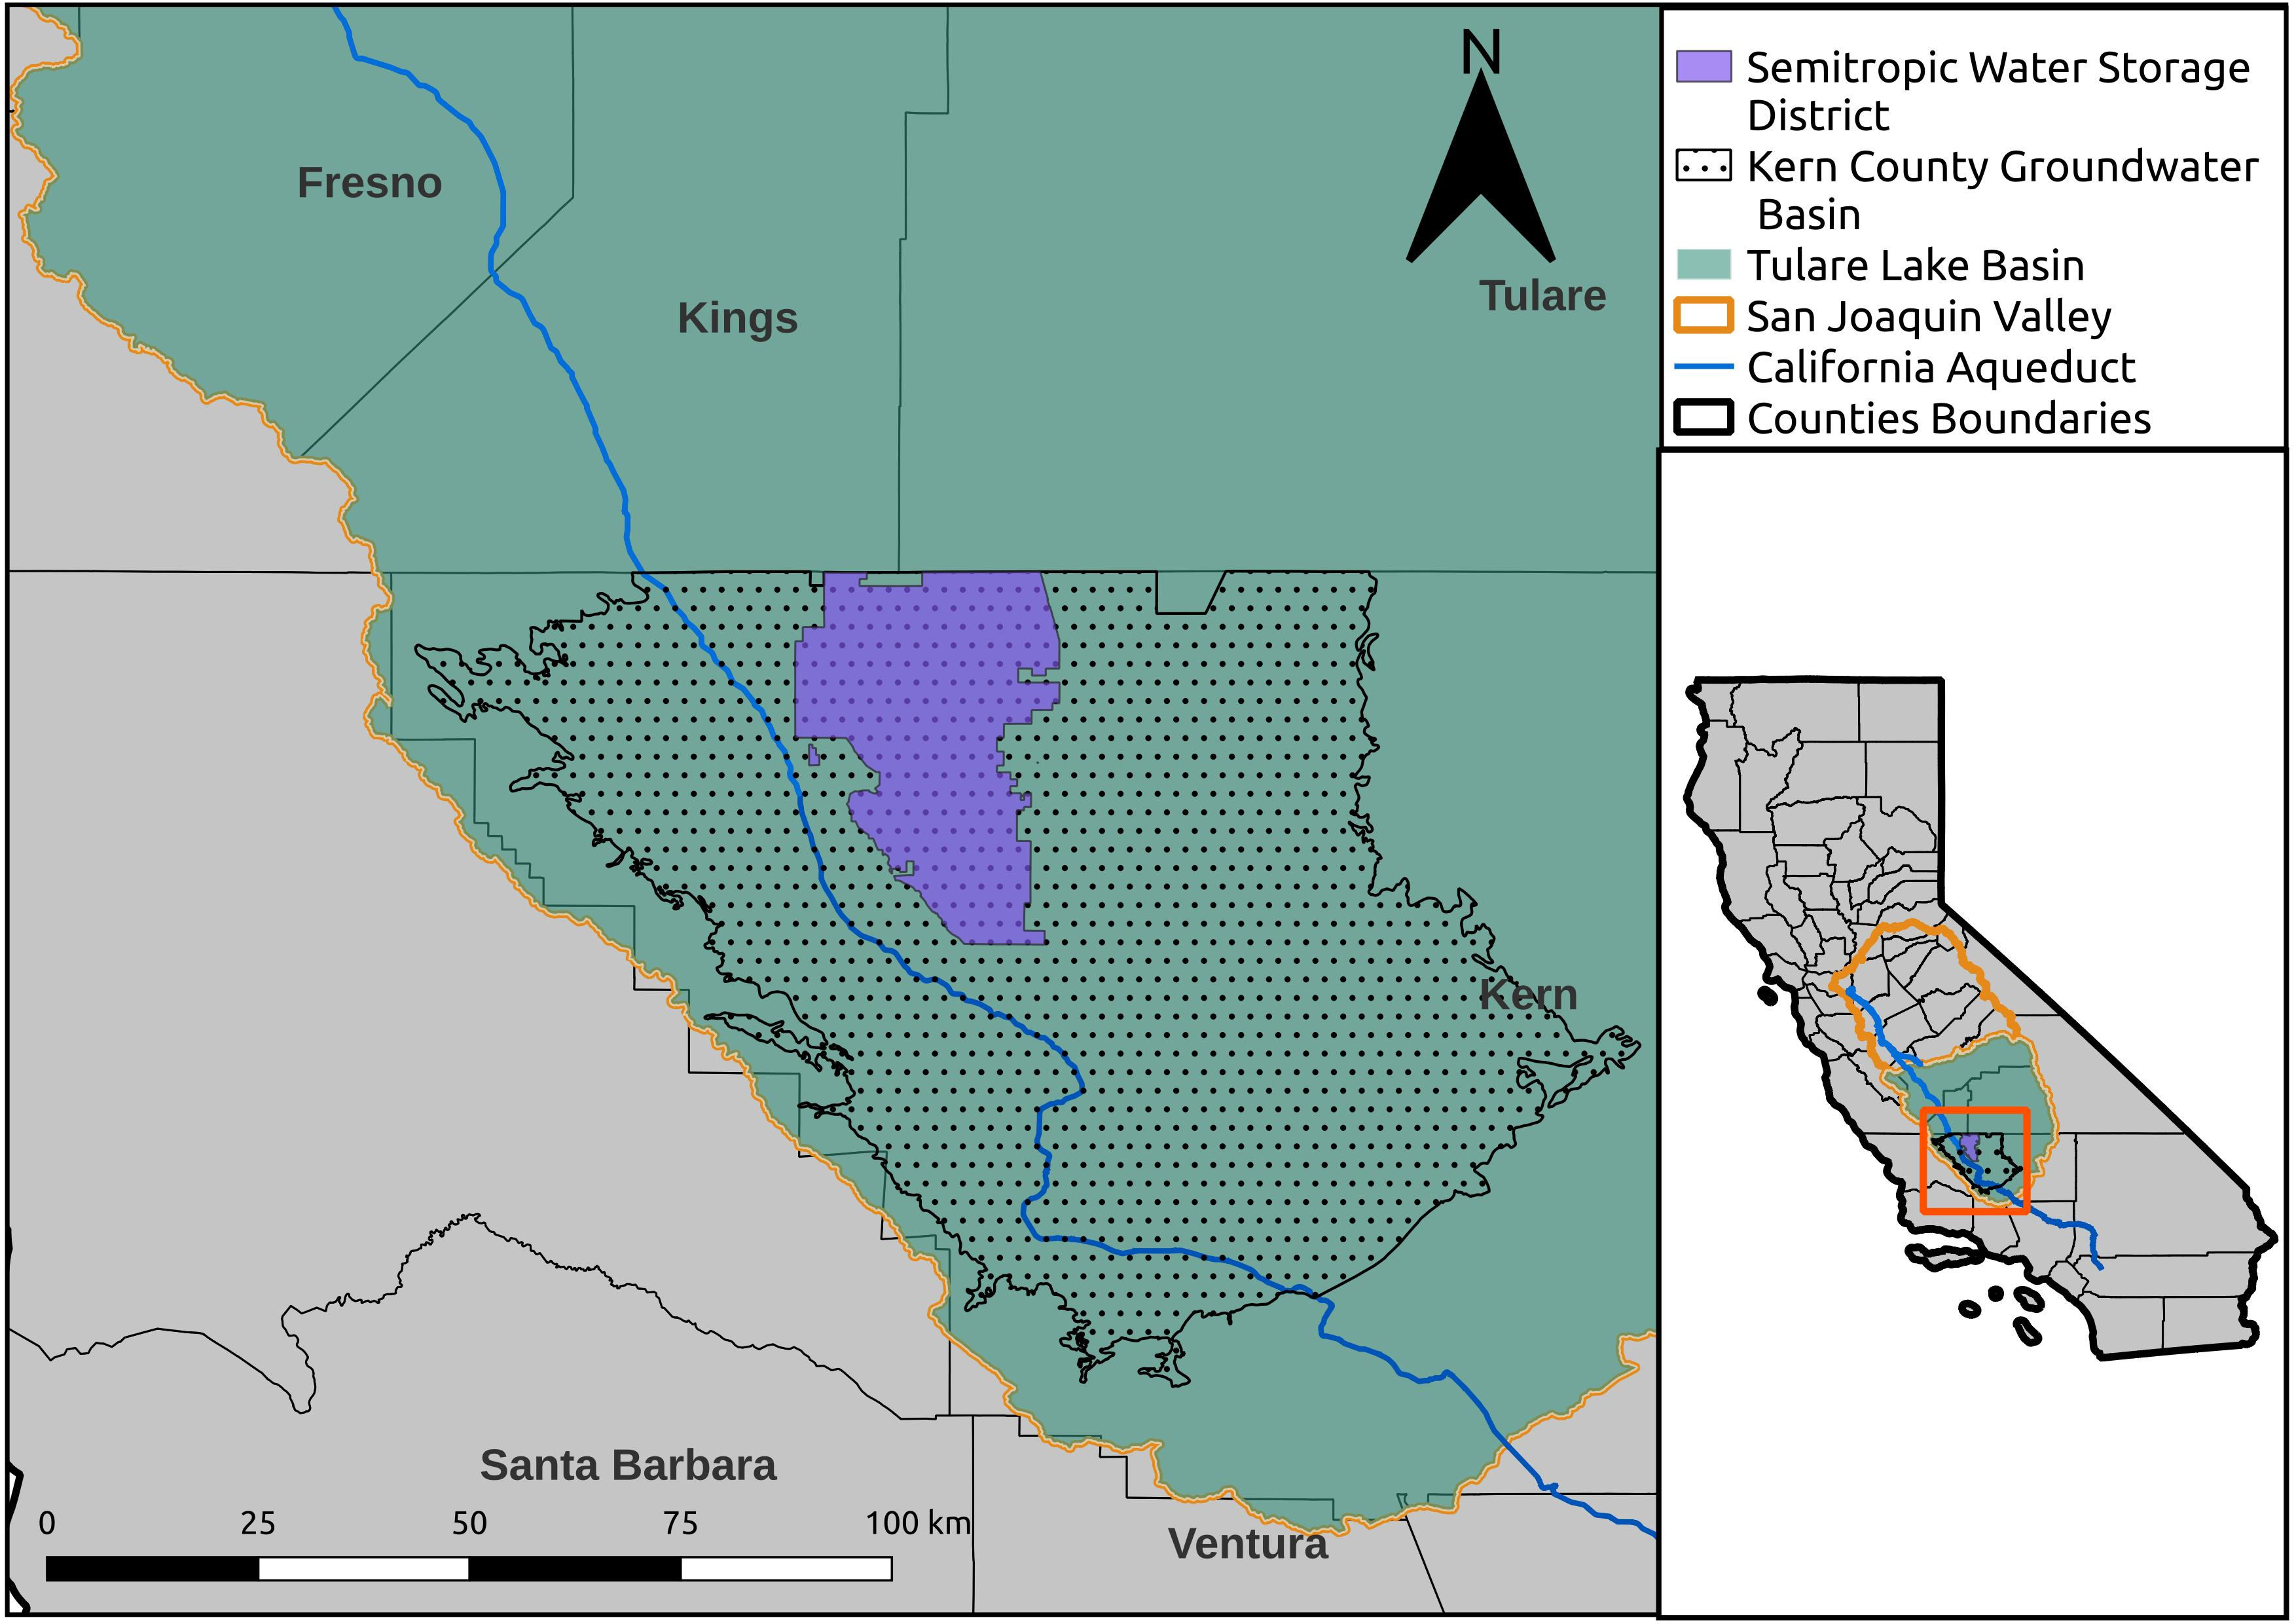
\includegraphics[width=0.8\textwidth]{Map_Semitropic.jpg}
    \caption{Semitropic Water Storage District study area located in the California’s San Joaquin Valley.}
    \label{fig:1}
\end{figure}

\subsection{Semitropic GSA Hydro-Economic model}

In food-water systems Hydro-Economic Models have been used as decision support modeling tools to assess water policy and climate change adaptation decisions (\cite{ward_hydroeconomic_2021,harou_hydro-economic_2009}). HEMs are able to abstract stakeholders decisions (e.g farmers) and hydrology dynamics, as well as their feedback, by integrating economic models with hydrological response functions (\cite{harou_hydro-economic_2009}). Given the modular characteristic of these coupled modeling methods is possible to assess the performance of economic revenues and aquifer dynamics, as shown by \textcite{macewan_hydroeconomic_2017}, \textcite{afshar_multi-objective_2020}, \textcite{rodriguez-flores_global_2022} and \textcite{graveline_combining_2020}. Additionally, these methods are flexible to assess the performance of water management policies, under different climate scenarios, and spatial and time scales.

\subsubsection{Economic model}

The food production system was modeled using a hydro-economic model (\cite{harou_hydro-economic_2009}) that can represent a yearly net profit maximization at the irrigation district level. With this economic model, we can model land and water (surface and groundwater) allocation decisions for crop production. This model assumes that farmers make production decisions to maximize their net revenues by considering crop prices, surface water availability, price of surface water, price of electricity and water management policies. We used a mathematical model based on Positive Mathematical Programming (PMP) (\cite{howitt_calibration_1995}), which uses a stochastic data assimilation method to calibrate the economic parameters described by \textcite{maneta_stochastic_2014} and \textcite{maneta_satellite-driven_2020}. This calibration framework enables the update of the distribution of the calibration parameters every time data becomes available. Appendix A provides more details on the calibration process. 

For the calibration of the model, we use statistical data from 1998 to 2015. After the last year of historical observations was incorporated in the recursive data assimilation process, the final ensemble with 400 samples of calibration parameters $\theta_{i} = [\mu_{i},\beta_{i,water},\beta_{i,land},\delta_{i},\lambda_{i,land},\lambda_{i,water},\bar{\lambda}_{land}]$ are used in the economic model. Equations 1-7 define the maximization problem that is nested in the MOEA for a Bi-level optimization problem (Section 3.2).

\begin{alignat}{1}
\underset{{\substack{x_{i,land,t}\geq0\\x_{i,water,t}\geq0\\wat_{i,w,t}\geq0}}}{max}& \sum_{i} \{p_{i,t} \mu_{i}(\beta_{i,land} x^{\rho_i}_{i,land,t}+\beta_{i,water} x^{\rho_i}_{i,water,t})^{\delta_{i}/\rho_i} - (\omega_{i,land} + \lambda_{i,land} + \bar{\lambda}_{land}) x_{i,land,t} \notag \\&-(\omega_{SW,t}+ \lambda_{i,water} )wat_{i,SW,t} - (\omega_{GW,t}+ \lambda_{i,water} + u^{GWF}_{t})wat_{i,GW,t}\}
\end{alignat}

\textit{subject to}
\begin{flalign}
&\sum_{i} x_{i,land,t} \leq u^{TL}_{t}& \\
&\underset{i\in{PC}}{\sum} x_{i,land,t}  \leq  u^{PL}_{t}\\
&\underset{i\in{PC}}{\sum} x_{i,land,t}  \geq \underset{i\in{PC}}{\sum} x_{i,land_{t\mh1}} * 0.95 \\
&x_{i,water,t} = wat_{i,SW,t} + wat_{i,GW_t} \\
&\sum_{i} wat_{i,SW,t} \leq b_{SW,t}   \\
&\sum_{i} wat_{i,GW,t} \leq u^{GWP}_t \\
& x_{i,water,t} \geq \bar{x}_{i,water}*0.98
\end{flalign}

Where Equation 1 represent the net revenue maximizing objective function, by allocating $x_{land,i}$, total water $x_{water,i}$, surface water $wat_{SW,i}$ and groundwater $wat_{GW,i}$ to each crop i (Figure S1). $p_{i,t}$ is the price per tonn of crop $i$. Crop production in the first term of Equation 1 is represented by a CES production function (\cite{debertin_agricultural_2012}), with the two inputs mainly land and water.  $\beta_{i,j=[land,water]}$ are the relative use of land and water. $\rho = (\sigma-1)/(\sigma)$ where $\sigma = 0.17$ is the elasticity of substitution following \textcite{howitt_calibrating_2012}. The scale parameter $\mu_{i}$ and $\delta_{i}$ are calibrated using the first order conditions (Appendix A). The rest of the parameters used in the linear costs are the calibrated Lagrange multipliers $\lambda_{water},\lambda_{land}$, associated to the observed water and land allocation per crop constraints respectively. Variable costs are linear and include cost of land ($\omega_{i,land}$) and the unit price of surface water ($\omega_{SW,t}$). In contrast the volumetric cost of groundwater pumping is given by $\omega_{GW,t}$, which is a function of price of electricity ($\omega_{E,t}$), the groundwater depth ($GWD_t$) and other parameters related to the characteristics of the wells (Appendix B). Additionally, a per cubic meter $u^{GWF}_{t}$ pumping fee can be implemented on top of the pumping cost.

The net revenue maximization problem is subject to resources availability and land and water quantitative controls provided by the constraints. Equation 2 is a total land restriction where $u^{TL}_{t}$ is the total land use control that can be implemented in a year $t$. Equation 3 is an upper boundary perennial crops restriction $u^{PL}_{t}$ that levers the expansion or reduction of land allocated to perennial crops, where $PC \in$ \{Almonds and Pistachios, Subtropical, Other Deciduous and Vine\}. In order to maintain the perennial crops removals to what has been observed historically we added a perennial removal constraint (Equation 4) to be no more than 5 percent of the land allocated to perennial removal. Equation 5 is a mass balance restriction where each crop can use water from both surface water and groundwater. Equation 6 is the surface water availability ($b_{SW,t}$) restriction. Equation 7 is the total groundwater pumping restriction where $u^{GWP}_{t}$ is the maximum allowed groundwater pumping decision. $u^{GWF}_{t}$, $u^{TL}_{t}$, $u^{PL}_{t}$, $u^{GWP}_{t}$ are the four management decision that this study assess formulated in the adaptive control policy (Section  3).  Finally, we allowed up to 2\% deficit irrigation through Equation 8 which allows reduction in the applied water per  unit of land ($\bar{x}_{i,water}$) with respect to baseline calibration conditions. 

\subsubsection{Groundwater Depth Response Function}

The dynamics of groundwater in the San Joaquin Valley depend on many geological, hydrological, climate and human components. To best represent the dynamics of groundwater depth level (potentiometric level) we used outputs from the physical based model Fine Grid California Central Valley Groundwater-Surface Water Simulation Model (C2VSIM-FG version 1.01) (\cite{dwr_c2vsimfg_2021}) to calibrate a response function. C2VSIM-FG has a finite element grid of more than 35,000 elements for California’s Central Valley California, and each element is able to link land surface, surface water and ground-water. The model employs historical data (i.e. cropland use, crop water demand, surface water diversions, precipitation, soil moisture), in the simulation process. C2VSIM-FG can be run for a simulation period from 1973 to 2015 at a monthly time step. Water budgets are generated for each element in the grid including groundwater pumping and groundwater depth and can be post-processed to create water budgets for defined boundaries (group of elements). We use the water budget generated for the Semitropic Water Storage District boundary. 

From C2VSIM-FG we used the weighted-average groundwater depth level to agricultural pumping to remove the elements where there is not agriculture within the district boundary. Since the economic model simulates farmers’ decisions at a yearly time step, we use the groundwater depth change from the beginning of the water year (October) to the end of the water year and irrigation season (September), and the total groundwater pumping in a water year to calibrate the response function. Figure 3 shows the simulated groundwater depth and agricultural pumping from C2VSIM-FG at the end of the water year. 

\begin{figure}[H]
    \centering
    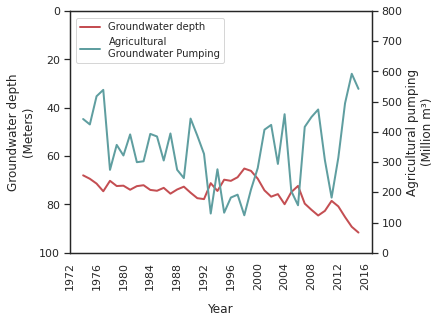
\includegraphics[width=0.5\textwidth]{c2vsim_semitropic.png}
    \caption{Groundwater depth and agricultural groundwater pumping from simulation outputs of C2VSIM-FG (\cite{dwr_c2vsimfg_2021})}
    \label{fig:mes1h1}
\end{figure}

The groundwater depth change response function was calibrated using a Bayesian linear regression (Appendix C). With this function we predict the groundwater depth change each year as a function of total agricultural pumping. As shown by Equation 9, the ground water depth level at the beginning of the year t ($GWD_{t}$) is calculated as the sum of the groundwater depth level at the beginning of the year t-1 ($GW_{t-1}$)  and the median of the predictive posterior distribution for groundwater depth change ($\overline{\Delta GWD}_{t-1}$) estimated at the end of the year t-1. By embedding this function into the economic model and by defining the pumping cost as a function of the groundwater depth (Appendix B) we are able to model the feed-back between food production and groundwater levels. 

\begin{align}
GWD_{t} = GWD_{t-1} + \overline{\Delta GWD}_{t-1}
\end{align}

\subsection{Stochastic time series}

To run the model dynamically, we build Monte Carlo time series for economic and hydrologic conditions that are used to force the HEM. Each time series starts at $t_{1}=2016$. In our analysis we included simulated surface water supplies to the irrigation district (Figure S2 in SI 3) from the California’s Food-Energy-Water System simulation model (CALFEWS) \cite{zeff_californias_2021}). These were simulated with down-scaled data from seven of the ten Global Circulation Models (GCMs) suggested by \textcite{pierce_climate_2018} (CCSM4, MIROC5, CanESM2, CNRM-CM5, GFDL-CM3, HadGEM2-CC and HadGEM2-ES), and using the Representative Concentration Pathway (RCP) 4.5 (moderate scenario) and 8.5 (high emissions scenario). 

Additionally, we considered uncertainties on economical variables and calibration parameters of the economic model, summarized in Table 1. Crop prices $p_{i,t}$ were sampled using the historical data from 1980 to 2020 (\cite{usda_national_2020}) and the price of electricity ($\omega_{E,t}$) was sampled from the historical (2008-2021) reported by the Pacific Gas and Electricity Company (PG\&E) for small and large agricultural users. The price of surface water ($\omega_{SW,t}$) was sampled from rates reported in the district using surface water supply to define water rates by water-year type category. All prices were adjusted for inflation using the consumer price index based on the year 2016. Finally a sample from the posterior distribution of the calibration parameters $\theta_{i}$ is sampled.

\begin{center}
\begin{tabular}{ |c|c|c|c| } 
 \hline
 Variable & Symbol & Units & Source \\ 
 \hline
 Crop prices & $p_{i}$ & \$/ton & \textcite{usda_national_2020}\\
 Price of electricity & $\omega_{E,t}$ & $\$/Kwh$ & \textcite{pge_pacific_2021} \\
 Price of surface water & $\omega_{SW,t}$ & $\$/m^3$ & Irrigation district reports\\
 Surface water supply & $b_{SW,t}$ & $m^3$ & \textcite{zeff_californias_2021}\\
 Calibration parameters & $\theta_i$ & - & Calibration process \\
 \hline
 \end{tabular}
\captionof{table}{Data Sources for Monte Carlo Time Series}
\end{center}


\section{Adaptive Dynamic Decisions}

Searching for adaptive groundwater management policies using DPS consists of finding parameters of the control policy function that optimized the trade-offs between groundwater sustainability and economic objectives. Different parametric functions can be used to model control policies, including linear, polynomial, neural networks, decision trees and radial basis functions (\cite{giuliani_universal_2014}). In this study we used cubic radial basis Functions (RBFs) to accommodate the complexity of the dynamic decisions that the GSA and farmers can coordinate given surface water supply, crop-land decisions, and groundwater depth at the beginning of the irrigation season. The four decisions that comprise the control policy are: Groundwater pumping fee (GWF), total land restriction (TL), perennial cropland restriction (PL) and groundwater pumping restriction (GWP). 


\subsection{Direct Policy Search}

Dynamic land and groundwater management decisions made at every year step $t$ are represented by the vector $u_{t}^D$ where $D \in \{GWP,TL,PL,GWF\}$ represent the four possible decisions. The control policy in Equation 10 equals to the outputs of a policy $P^D$ which is a mathematical function with two vector inputs: the structural parameters of the RBFs ($\psi^D$) and system-state information vector ($I_{t'}$). Information variables in $I_{t'}$ represent key components of the food-water system which values can be from the current year $t$ or previous year $t-1$. 

\begin{align}
u_{t}^D = P^{D}(I_{t'}|\psi^{D})
\end{align}

In direct policy search, the use of RBFs have shown to be an efficient way to represent complex decision making. These have been applied to lake pollution control (\cite{quinn_direct_2017}), reservoir operation (\cite{giuliani_universal_2014, zatarain_salazar_balancing_2017}), sea-level rise protection (\cite{garner_using_2018}), and financial risk management in water-energy systems (\cite{gupta_can_2020,hamilton_stream_2022}). For this study we define the control policy function $P^D$ as set of cubic radial basis functions given by Equation 11.

\begin{align}
u_{t}^D = \phi^{D}\left(\sum_{m=1}^M w_{m}^D \sum_{j=1}^J \left\lvert\dfrac{[I_{t'}]_{j}-c_{j,m}}{r_{j,m}}\right\rvert^{3}\right)
\end{align}

Where $\phi^{D}$ is an outer function, $w_{m}^D$ is the weight of M cubic radial basis functions. The weights can have values $ 0 \leq w_{m} \leq 1$ and are subject to $\sum_{m=1}^M m_{m}^D= 1$. The four decisions in the control policy share the same RBFs structure; hence the information vector $I_{t'}$ is shared for all decisions. Additionally, $c_{j,m} \in [-1,1]$ and $r_{j,m} \in (0,1]$ are the center and radius respectively shared by all the RBFs. $I_{t'}$ in Equation 12 is a vector with system state variables that inform the policies, where $\overline{GWD}_{t}$ is the normalized level to groundwater at the beginning of the year, $\overline{PCL}_{t-1}$ is the normalized area devoted for perennial crops production in the year $t-1$. $\overline{b}_{SW,t}$ is the normalized surface water available in year $t$. Normalization was performed using $k^{GWD}$, $k^{TL}$, $k^{SW}$ to obtain $\overline{GWD}_{t}$, $\overline{PCL}_{t-1}$, $\overline{b}_{SW,t}$ respectively summarized in Table 2.

\begin{align}
I_{t'} = [\overline{GWD}_{t},\overline{PCL}_{t-1},\overline{b}_{SW,t}]
\end{align}

The function $\phi^{D}$ in Equation 11 can consist on two functions, unnormalize $\phi^{D,N}$ and constraint $\phi^{D,C}$, used to obtain the values of the management decisions in the control policy $u_{t}^D$. Being $z_{t}$ the argument in the $\phi^{D}$ function (Equation 11), the value of each decision is defined by the following equation.

\begin{align}
u^{D}_t = \phi^{D,C}(\phi^{D,N}(z_{t}))
\end{align}

For the groundwater pumping restriction policy ($u^{GWP}_t$) $\phi^{GWP,N}$ scales the groundwater that farmers will have available to pump between zero and the pumping capacity of the district $k^{GWP}$ (maximum observed pumping). $\phi^{GWP,C}$ constraints the groundwater pumping to be at least the difference between the water demand by perennial crops of the year $t-1$ and the surface water available in the year $t$. 

\begin{align}
z'_{t}=\phi^{GWP,N}(z_{t}) = k^{GWP}max(min(z_{t},1),0) 
\end{align}

\begin{align}
u^{GWP}_t = \phi^{GWP,C}(z'_{t})= max(z'_{t},\underset{i \in PCL}{\sum} x_{i,water_{t\mh1}} - \; b_{SW,t})
\end{align}

In Equation 16 the unnormalize function ($\phi^{TL,N}$) scales the total land decision that farmers can produce in the district for the year t, between zero and $k^{TL}$, where $k^{TL}$ is the total land in the district (maximum observed produced land). As shown in Equation 15, $\phi^{TL,C}$ constraints the total land decision to be at least the land used by perennial crops in the the year $t-1$.

\begin{align}
z'_{t} = \phi^{TL,N}(z_{t}) = k^{TL}max(min(z_{t},1),0)
\end{align}

\begin{align}
u^{TL}_t = \phi^{TL,C}(z'_{t})= max(z'_{t},\underset{i \in PC}{\sum} x_{i,land_{t\mh1}})
\end{align}

For the perennial crops planting restriction ($u^{PL}_t$), $\phi^{PL,N}$ scales the total land that can be allocated to perennial crops between zero and the total land available in the district ($k^{TL}$). $\phi^{PL,C}$ constraints the perennial restriction to be at least 95\% of the previous year perennial crops land, and it limits the expansion of perennial crops to 5\% more acreage from the previous year $t-1$. These restrictions are applied to ensure that solutions of the control policy are realistic to what has been observed the region.

\begin{align}
z'_{t} = \phi^{PL,N}(z_{t}) = k^{TL}max(min(z_{t},1),0)
\end{align}

\begin{align}
u^{PL}_t = \phi^{PL,C}(z'_{t})= \begin{cases}
      \underset{i\in{PC}}{\sum} x_{i,land_{t\mh1}}*1.05,  \text{\; if \, $z'_{t}$  $>$ $\underset{i\in PC}{\sum}x_{i,land_{t\mh1}}*1.05$}\\
       \underset{i\in PC}{\sum} x_{i,land_{t\mh1}}*0.95, \text{\; elif \, $z'_{t}$  $<$ $\underset{i\in PC}{\sum}x_{i,land_{t\mh1}}*0.95$}\\
      z'_{t}, \text{\; $otherwise$}
\end{cases}     
\end{align}

Finally for the pumping fee ($u^{GWF}_t$), the function $\phi^{GWF}$ in Equation 20, scales the groundwater pumping fee that can have values between [0,$k^{GWF}$]. $k^{GWF}$ is set to be $\$0.5/m^3$, hence the upper boundary of the pumping fee is 0.5 USD per cubic meter. This fee sums to the groundwater pumping cost in the objective function of the economic model (Equation 1).

\begin{align}
u^{GWF}_t = \phi^{GWF,N}(z_{t}) = k^{GWF}max(min(z_{t},1),0)
\end{align}

The dynamic control policy is represented by the set of Equations 11 to 20, where the vector of structural parameters $\psi = [w^{D},c,r]$ of the RBFs is optimized. Since the information vector $I_{t'}$ of size $J$ is shared across decisions in $M$ number of RBF's the vectors of centers (c) and radii (r) are equal to $c=[c_{0,0},...,c_{J,M}]$ and $r=[r_{0,0},...,r_{J,M}]$.


\begin{center}
\begin{tabular}{ |c|c|c|c| } 
 \hline
 Variable & Symbol & Units & Value \\ 
 \hline
 Normalization for cropland  & $k^{TL}$ & $Kha$ & 62\\
 Normalization for groundwater pumping & $k^{GW}$ & $M m^3$ & 732 \\
 Normalization groundwater depth  & $k^{GWD}$ & $m$ & 198 \\
 Normalization for pumping fee   & $k^{GWF}$ & \$/$m^3$ & 0.5 \\
 Normalization surface water  & $k^{SW}$ & $M m^3$ & 208 \\
 \hline
 \end{tabular}
\captionof{table}{Normalization factors used in the control policy}
\end{center}


\subsection{Bi-level Optimization Problem}

This study implements two optimization processes (Figure 4). A MOEA is used to optimize the vector of structural parameters in the RBFs ($\Psi$). Each set of structural parameters define a control policy (Section 3.1) or set of decisions ($u^{D}$) which are assessed in the Hydro-economic model (Section 2.1) using N Monte Carlo realizations with times series of T years (Section 2.2). Hydro-economic model then finds optimal land and water allocation for the first five years of each time series resolution. Thus at t=5 the model starts the implementation of management decisions and the assessment of objectives. This was done to simulate flexible groundwater management described in Section 1 and Figure 1. The results of the process are aggregated in five performance metrics, representing the groundwater sustainability and economic goals of the GSA. The value of the objectives and constraints from the candidate policy assessment feedback to the MOEA to continue its optimization process. 

\begin{figure}[H]
    \centering
    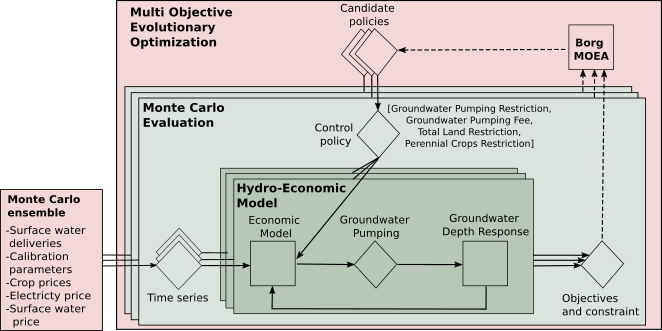
\includegraphics[width=0.9\textwidth]{Diagram2}
    \caption{Bi-level optimization problem schematic adapted from \textcite{hamilton_stream_2022}. Rectangles represent the modules that contain optimization and simulation models (squares) and inputs/outputs (diamonds). Dashed arrows depict the Borg MOEA feed-back process where the values of objectives and constraint are from performance metrics of the Hydro-economic model  result of an implemented control policy.}
    \label{fig:m1esh1}
\end{figure}

The first level optimization consists in a multi-objective evolutionary optimization where five objectives are minimized or maximized, the decision variables are the structural parameters of the RBFs in the vector $\Psi$, used to parameterize the control policy. 

\begin{align}
\underset{\Psi}{argmin} = (-O_{1}(\Psi),O_{2}(\Psi),-O_{3}(\Psi),O_{4}(\Psi),-O_{5}(\Psi))
\end{align}

The first objective $(O_{1})$ is to maximize the average total revenues $\pi_{n,t}$  from the average total net revenue of N ensemble realizations with T years. This objective represents the economic objective of farmers of revenue maximization. A lower boundary constraint for this objective is defined to achieve at least an average total revenue greater or equal than \$11 billion. This restriction constrains the algorithms from finding unrealistic policies far from farmers preferences. 

\begin{align}
O_{1} = \frac{1}{N}\sum_{n=1}^N(\sum_{t=5}^T \pi_{n,t})
\end{align}


\begin{align}
O_{1} \geq 11,000
\end{align}

The second objective is the minimization of the average groundwater depth. The average groundwater depth is calculated over the years of management implementation implementation (T-5) for each Monte Carlo realization, and then the average of these are taken over all the N Monte Carlo realizations. 

\begin{align}
O_{2} = \frac{1}{N}\sum_{n=1}^N(\frac{1}{T-5}\sum_{t=5}^T GWD_{n,t})
\end{align}

The third objective is to maximize the 5th percentile of minimum profits. This metric represents a \textit{max-min} goal, used to inform decision makers about the of the worst profits in a given year. Even though there are economic factors included in the stochastic ensemble that can be drivers of low economic revenues, management decisions can be the main causes of expected low profits particularly during dry years, as shown by \textcite{rodriguez-flores_global_2022}. 

\begin{align}
O_{3} = Q5_{N} \bigg[\underset{t\in(5,...,T)}{min}[\pi_{n,t}]\bigg]
\end{align}

The fourth objective is to minimize the 95th percentile of maximum groundwater depths. This objective represents a \textit{min-max} goal of the largest groundwater depth. The maximum groundwater depth level is taken over each implementation period and the Q95 operator takes the 95th percentile over all N the Monte Carlo  realizations. 

\begin{align}
O_{4} = Q95_{N} \bigg[\underset{t\in(5,...,T)}{max}[\overline{\Delta GWD}_{t-1}]\bigg]
\end{align}

As explained in the Introduction during dry years the groundwater depth can go above the measurable objective, with the expectation that in wet years it will recover. However, the objective is to maximize the number of years that the groundwater depth is at most at the measurable objective level, limiting the groundwater level to go above the minimum threshold. Thus, the fifth objective is to maximize the average fraction of years (reliability) that the distance to the groundwater depth bellow or at the measurable objective ($GWD^{SGMA}$). We used the 2015 groundwater level from C2VSim-FG as a measurable objective as it was the deepest year in the recent 2012-2016 drought (Lund et al. 2018). Additionally, we included a constraint (Equation 28) that the reliability must be at least 20\% (i.e. one of every five years). 

\begin{align}
O_{5} = \frac{1}{N(T-5)}\sum_{n=1}^N(\sum_{t=5}^T \tau_{n,t})\; where\; \tau_{n,t} = \begin{cases}
      1, \text{\; $GWD_{n,t}$  $\leq$ $GWD^{SGMA}$}\\
      0, \text{\; $GWD_{n,t}$ $>$ $GWD^{SGMA}$}\\
\end{cases}      
\end{align}


\begin{align}
O_{5} \geq 0.2
\end{align}

\subsection{Robustness Analysis}

Solutions in the Pareto front are each distinct control policies that prioritize a subset of objectives. Stakeholders can then choose acceptable policies based on their preferences. However, it is important that the policies can perform well in alternative states of the world that they aren’t optimized to. Thus, we reevaluate these policies across a broader sampling of deep uncertainties (Section 2.2) to quantify their robustness. Different metrics can be used to measure the robustness of each control policy which inherently represents a variety of farmers’ and water managers’ acceptability thresholds and their perception of risk (\cite{mcphail_robustness_2018}). For this study we selected the domain criterion satisfying metric  (\cite{schneller_decision_1983}) that quantifies the fraction of scenarios (rate of success) that achieve a minimum performance threshold, defined by stakeholders, from a larger set of states of the world different than the ones used in the EMODPS search. 



\section{Computational Experiment}

The search for  optimal RBFs parameters in EMODPS is a non-convex problem (\cite{giuliani_curses_2016}) that can be solved using heuristic methods. MOEAs are a popular tool for multi-objective optimization that iteratively improve a population of possible solutions  until the population reaches a stable Pareto front or set of  non-dominated solutions (\cite{coello_evolutionary_2007}). The solution space associated with this formulation is highly complex and characterized by characterized by a topology that nonlinear and non-convex. Thus, it is important to use the appropriate MOEA that is capable of searching such complex topologies. For this study we use the Borg MOEA (\cite{hadka_borg_2013}), a self-adaptive algorithm that employs probabilistic operators as $\epsilon$-dominance, adaptive population sizing and time continuation through $\epsilon$-progress. Borg MOEA has shown have better time efficiency, scalability, and controllability, as well as less sensitivity to its parameterizations compared to other MOEA algorithms (\cite{reed_evolutionary_2013,gupta_can_2020,zatarain_salazar_balancing_2017}). Since Borg MOEA is a stochastic algorithm we estimate Pareto-front solutions using ten different random seeds (i.e.  random initializations of the population) using the master-worker parallel configuration of Borg (\cite{hadka_large-scale_2015}). $\epsilon$-values (resolution) for each objective are summarized in SI Table S2. 


The economic model (Equations 1-8) was formulated using the Python package Pyomo (\cite{hart_pyomo_2011}) and solved using the non-linear programming solver IPOPT (\cite{wachter_implementation_2006}). The decision variables in the economic model are the allocation of land and water (surface water and groundwater) to seventeen crop groups resulting for a total of 68 decision variables for each time step t. Additionally at each time step a posterior predictive sample of groundwater depth change with 400 samples was estimated using the model results and trace generated using the probabilistic programming Python package PyMC  (\cite{salvatier_probabilistic_2016}).

We performed the bi-level optimization process for an ensemble of N = 100 Monte Carlo realizations and T = 30 years for 50,000 candidate policy trials (function evaluations). A structure of M=4 RBFs (Equation 11) was selected given its good performance, resulting in 40 decision variables in the vector  $\Psi$ to be optimized with Borg MOEA. The final Pareto-set solutions was selected from the random seed with the highest hypervolume (\cite{hadka_large-scale_2015,reed_evolutionary_2013}), shown in the Figure S10 of the SI. The selected Pareto-set was later assessed in a larger set of Monte Carlo ensemble of N = 400 to inform the robustness analysis. One limitation of the bi-level optimization is the high computational demand that limited the number of Monte Carlo resolutions and function evaluations, however as shown the random seeds hypervolume performance they converged around half of the 50,000 evaluations. All the computational experiments were performed in the MERCED cluster of the University of California Merced. 


\section{Results and Discussion}

Figure 5 shows  Pareto-approximate reference set that spans different trade-offs among the five objectives in the problem. In the figure each triangle represents the objective values associated with selected control policies ($\Psi$ values). The size of the triangle depicts the 95th percentile of the maximum groundwater depth changes in a year, and the color gradient depicts the 5th percentile of the minimum revenue in a year. The star represents a hypothetical the ideal solution that would allow for the shortest average groundwater depth while providing the highest possible revenue across the sustainable management implementation period. Characteristic behavior emerges particularly as average groundwater depth decreases, economic revenues (and minimum revenues) decrease as well. Average groundwater depth decreases also correspond to an increase in reliability. However, for some policies to attain one hundred percent reliability, they must rely on limiting the pumping that agriculture is using, including during dry years, which results in lower total and minimum revenues. These solutions represent decisions that are unlikely to be applied in the water district as achieving the measurable objective all the years is not the objectives of flexible management. Maximum groundwater depth change (size of the triangle) reach values as the maximum depth change observed in the historical record (Figure S7), highlighting the capacity of the policies to avoid larger depth changes even in drier future conditions. However, as maximum depth changes reduce the Pareto-set shifts downwards resulting in lower average revenues. 

\begin{figure}[H]
    \centering
    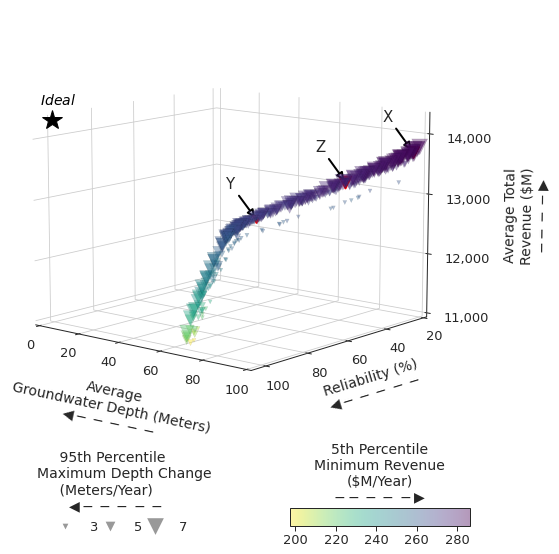
\includegraphics[width=0.8\textwidth]{selected_policies_3d.png}
    \caption{Pareto approximate set from the EMODPS experiment} \label{fig:parallel_robustness}
\end{figure}

To assess the adaptive capacity of the resulting policies to uncertain future system conditions and uncertain surface water supplies, we selected three policies that achieve various levels of reliability. Policies X, Y, and Z prioritize different sets of objectives summarized in Table 3. These control policies  were run with four management decisions that can be  chosen each year before the irrigation season starts, for a 25 years of policy implementation. We selected a state of the world with the largest standard deviation on surface water deliveries (CANESM2 8.5) due to its good representation of the region characteristics with dry periods with wet years in between. As in the experiment we let the model to run five years with no management policies starting the implementation of decisions at t=5. 

\begin{center}
\begin{tabular}{ |c|c|c|c|c|c| }
 \hline
 Solution & O1 & O2 & O3 & O4 & O5 \\ 
 \hline
X &  13,718 & 98.14 &  285 & 4.9 & 22\% \\
Y &  13,053 & 87 & 267 & 3.6 & 90\% \\
Z &  13,381 & 91.7  & 277 & 5.3 & 50\% \\
\hline
\end{tabular}
\captionof{table}{Performance of the selected policies shown in Figure 5}
\end{center}

Figure 6 shows the evolution of dynamic management decisions and their performance in the food-water system. Before the management policies were implemented perennial cropland expanded relying on pumping due to reduced surface water (a), increasing the groundwater depth (g). Starting with implementation (after year 5), Figure 6 shows how decisions ((b) to (e)) evolve, showing the adaptive dynamic performance of the control policy. The total land planting decision (e), is the only decision that shows a non-implementation behavior, given that other decisions regulate land use via groundwater pumping that result in a better performance of the system. In general, similar behavior is shown by the experiments across the other three decisions in the selected control policies, however depending on where the solution is in the approximate Pareto-set, the magnitude of the decisions changes. Figure 6 panel (b) demonstrates that all three solutions implement groundwater restrictions during the initial stages of management and during dry years. Additionally, policies show a declining land allocation to perennial crops by 40\% of the initial area (i). This result confirms that sustainable groundwater management benefits from reducing the hard water demand imposed by perennial tree crops which has also been suggested in other studies (\cite{qin_flexibility_2019,mall_water_2019}). 

During dry years, control policies allow pumping to offset lack of surface water, however such policies do not reach the region’s pumping capacity and limit pumping to be extracted at a threshold, which can be considered a safe yield as shown by \textcite{miro_framework_2019} and \cite{macewan_hydroeconomic_2017}. In Figure 6 panel (f) shows that at t=10, when perennial tree crops have been reduced by the perennial planting decision, the control policy regulates most of the planting via a groundwater pumping fee (c). Control policies establish a pumping fee for all the implementation period, however use of a pumping fee peaks during wet years to limit the expansion of annual crops and maximize groundwater recovery. Implementing a pumping fee can improve the irrigation efficiency and control the expansion of cropland during wet and dry years as suggested by \textcite{stone_economic_2022}, \textcite{graveline_combining_2020}, and \textcite{khan_effect_2019}. The examined policy solutions suggest a pumping fee between $\$0.1/m^{3}$ and $\$0.2/m^{3}$ that increases up to $\$0.5/m^{3}$ during wet years incentivizes sustainable pumping and maximizes groundwater recovery. Additionally, control policies manage annual crops planting (j) to work as a flexible land use where at the beginning of implementation these crops reach its lowest level to allow a rebound of the groundwater level and after that they are regulated in a flexible way between wet and dry years. However, total land in annual crops decisions indicates lower levels compared to the baseline even in wet years as suggested by \textcite{hanak_water_2019}. 

\begin{figure}[H]
    \centering
    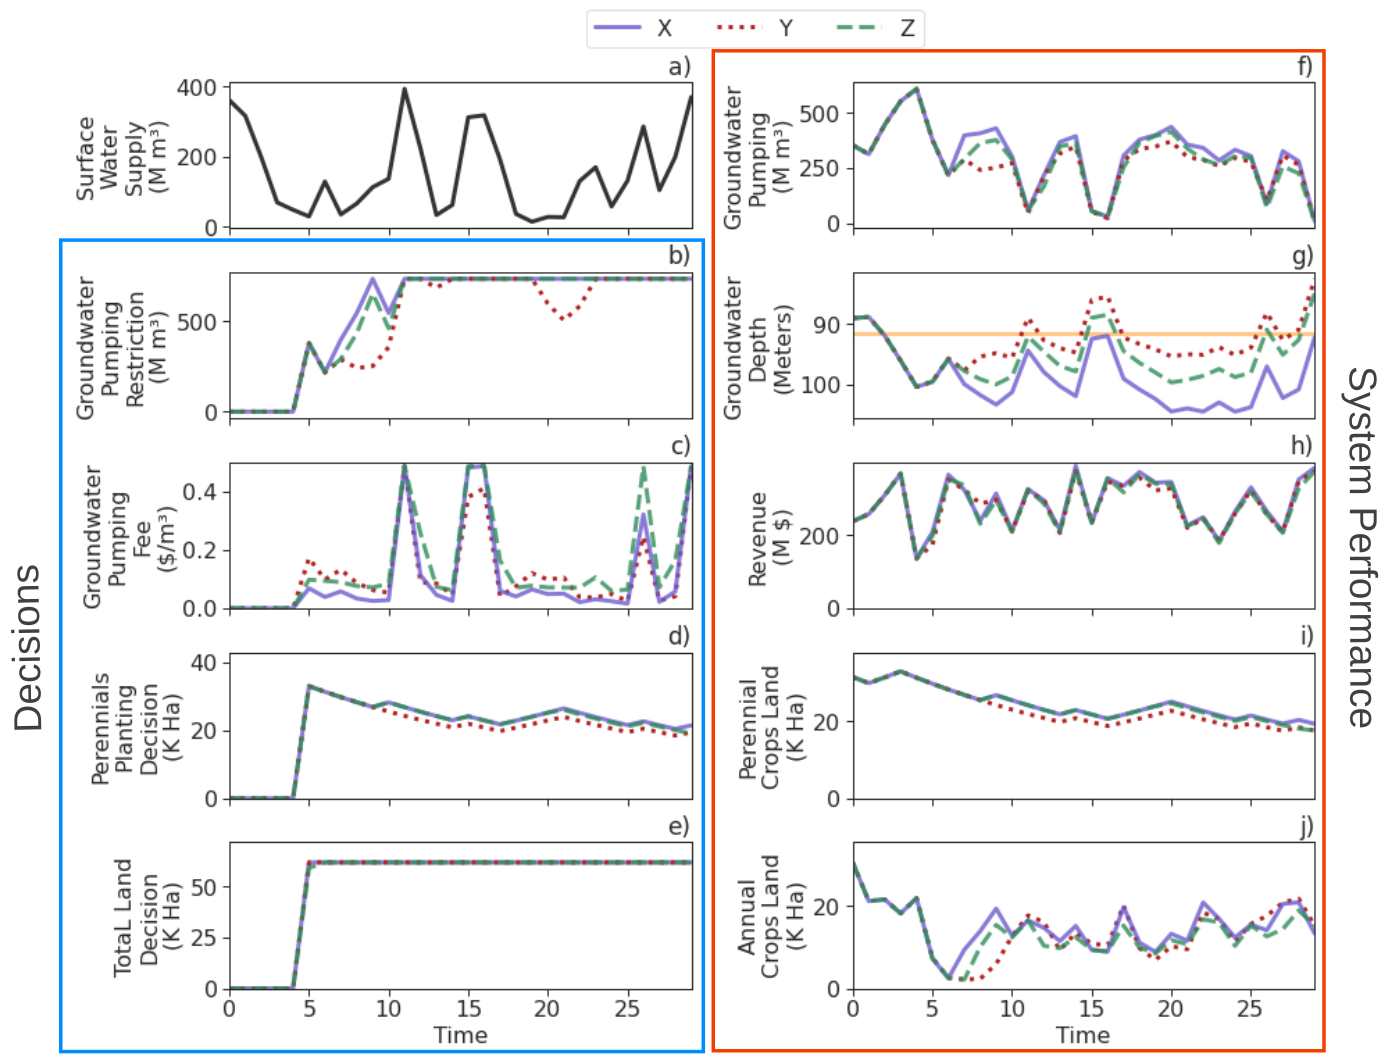
\includegraphics[width=1\textwidth]{selected_policies_performance_labels.png}
    \caption{Performance of the dynamic policies and hydro-economic model over a 30 year realization period with 25 five years implementation of land and groundwater management decisions. Sub-figure (a) shows the surface water deliveries.Sub-figures (b) to (e) show the dynamic decisions in the control policy. Sub-figures (f) to (j) show the performance of the food-water system. The orange line in Sub-figure (g) depicts the measurable objective used in the experiment.} \label{fig:parallel_robustness}
\end{figure}

Selecting different solutions along the Pareto approximate set allows assessment of their performance and provides insight of potential trade-offs of implementing management decisions. As shown in Figure 6 (g) implementing the control policy Y results in a lower average groundwater depth and larger number of years where the "measurable objective" (yellow line) is met. However, solutions X and Z achieved the measurable objective in wet years and prescribe higher cropland than solution Y. One key insight is that control policies stopped the decline in groundwater depth observed in the historical record (Figure 2), allowing the groundwater depth to reach a maximum depth level where is feasible to recover and from where is able to meet the measurable objective in wet years. Depending on the control policy, the maximum depth level ("minimum threshold") and the number of years that achieve the measurable objective change. This suggests GSAs can maintain the groundwater depth below the minimum threshold and this level conditions the recovery capacity and number of years that the measurable objective is achieved post-drought. However, policies need to be flexible enough to allow groundwater depth to recover during wet years contrary to what has been observed during the last decade (\cite{liu_groundwater_2022,alam_post-drought_2021}).

\subsection{Robustness Analysis}

As shown, different policies can result in different system performances, and selecting policies for further exploration can be difficult given the large set of solutions. However, by performing a robustness analysis we can filter the solution space to focus on policies that meet desirable minimum criteria, measurable objective, and economic goals that the GSA and farmers define. We assessed the Pareto set in Figure 5 with N=400 Monte Carlo resolutions each with T=30 years. Each time series has a set of surface water supplies, crop prices, electricity price, surface water price and calibration parameters (Section 2.2). To illustrate this process, we defined an example of performance criteria and rates of success, shown in Table 4, all of which a control policy must achieve in N resolutions times 25 years of management implementation to be considered robust. These performance criteria include a measurable objective and minimum threshold or maximum groundwater depth that should be reached in a year. Additionally, a minimum perennial trees land in a year is defined to be at least 50\% from the baseline (33,161 ha). 

\begin{center}
\begin{tabular}{ |c|c|c|c| }
 \hline
 Criteria  & Threshold & Units & Rate of Success \\ 
 \hline
Minimum Revenue in a year  & > 270 & M USD & $\geq$ 70\% \\
Minimum Total Revenue   & > 12,500 & M USD & $\geq$ 80\% \\
SGMA Objective Reliability & < 91.4 & m bls & $\geq$ 20\%  \\
Minimum Threshold Reliability  & < 115 & m bls & $\geq$ 99\%  \\
Minimum Perennial Trees Land in a year  & > 16,580 & hectares & $\geq$ 90\%  \\
\hline
\end{tabular}
\captionof{table}{Performance Criteria for selection of robust policies}
\end{center}

Following these criteria we found twelve robust solutions out four hundred twenty six in the reference Pareto-set (Figure 7). These polices can be further explored to assess their performance under states of the world that can be of interest of stakeholders. To continue this exploration we selected two policies from the set of twelve robust policies: the policy with the largest total average revenue and the one with the lowest average groundwater depth from the 400 Monte Carlo resolutions. The performance of these robust policies was later assessed using the using the surface water deliveries with highest standard deviation (Figure S12), lowest average surface deliveries (Figure S13) and largest average deliveries (Figure S14). Results can be found in SI 8, where we show that even in the driest conditions robust policies are able to stop the positive rate of ground water depth increase, implementing adaptive policies that maintain the depth level within a margin of operational flexibility defined in the robustness criteria and achieving the measurable objective in wet years. 

\begin{figure}[H]
    \centering
    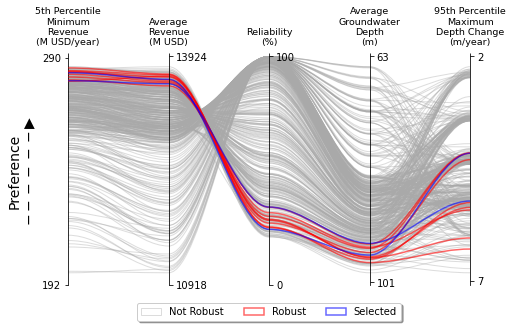
\includegraphics[width=0.7\textwidth]{robust_policies_parallel_axis.png}
    \caption{Policies from Pareto approximate set shown Figure 5. Robust policies are in red and selected robust policies for further analysis in blue. Policies in the Pareto-set that did not meet the satisfying criteria are in grey.} \label{fig:parallel_robustness}
\end{figure}

\section{Discussion}

This study contributes a novel assessment of the suitability of evolutionary multi-objective direct policy search to discover adaptive groundwater management strategies with a focus on meeting SGMA sustainable groundwater guidelines. We assess the ability of EMODPS to help operationalize groundwater sustainable management that targets the yearly decisions of water managers and farmers within both sectors of the complex food-water system. Resulting policies were adaptive to changes in system conditions, showing flexibility between dry and wet years, that maximize total average revenue and lowest revenue in a year and minimize average groundwater depth and maximum groundwater depth in a year. This paper contributes to the body of literature that evaluates optimal land and water use controls and economic instruments (e.g. pumping fees) to achieve groundwater sustainability in agriculture. To the authors’ knowledge, this is the first paper to search for dynamic adaptive policies in food-water systems.  

This study was applied to the Semitropic Water Storage District GSA in Kern County, California, which represents a broad set of water agencies in overdrafted groundwater basins subject to groundwater sustainability legislation. Results from this study provide insight into the ongoing development and implementation of groundwater management policies which can be scaled up to other basins agencies in the state. Overall, we find that:  

\begin{enumerate}
    \item   Reducing the proportion of perennial trees improves the adaptation capacity by increasing water demand flexibility.  
    \item  Annual crops can work as a buffer to support cropland increases during wet years and reductions during dry years.
    \item  Additionally, in early groundwater management implementation, a groundwater restriction is needed to bring the groundwater depth to a level where GSAs can feasibly manage groundwater to achieve measurable sustainable groundwater depth.
    \item  A pumping fee policy shows promise in coordinating surface and groundwater use and incentivize sustainable pumping. 
\end{enumerate}

This study used the sustainable management criteria defined by the California’s 2014 Sustainable Groundwater Management Act to assess the policies found by the EMODPS. Such policies allow a margin of operational flexibility where the groundwater depth can reach a sustainable objective, defined in this study, allowing an increase in groundwater depth during dry years but where is still feasible its recovery. However, as showed in this  study the capacity of a GSA to achieve this management depends on the minimum depth threshold and the capacity to decrease the irrigation demand in dry years and maximize recharge during wet years. The methodology shown in this paper can be applied to other agricultural regions in the world where irrigation is the main groundwater user and finding adaptive policies is crucial for groundwater sustainability. 

\subsection{Limitations and Future Work}

Climate change impacts in the region such as impacts on crop yields (\cite{blanc_is_2017}) and increase on potential evapotranspiration (\cite{mcevoy_projected_2020,vahmani_will_2022}) may occur but were not part of the present analysis. Additionally, surface water deliveries used in this study were obtained from the CALFEWS model (\cite{zeff_californias_2021}) which may have other intrinsic uncertainties not discussed in this study. Also, the groundwater depth response employed does not reflect the complexity of the aquifer dynamics, such as lateral flows from nearby basins, and surface-groundwater interactions beyond agricultural recharge among others. However, the groundwater response approach employed allows us to capture the general trend and response from groundwater pumping and recovery in the district. Crop prices used in the computational experiment were sampled from the historical and may not reflect future conditions, which are difficult to forecast given their variability and dependence on a highly dynamic globalized economy. 

Future studies could consider increase groundwater via managed aquifer recharge (\cite{alam_can_2020}) and potential participation in water markets (\cite{arellano-gonzalez_adaptive_2021,hanak_water_2019}) that can potentially increase the water availability and groundwater recovery. The results demonstrate that cropland reduction is a feasible strategy to achieve groundwater sustainability. However, developing cropland repurposing frameworks that can benefit groundwater sustainability, ecosystems and communities could have synergistic positive economic outcomes (\cite{biggs_landowner_2022,fernandez-bou_water_2023}). The multiple benefits from repurposing cropland could be included as additional objectives along with objectives that relate to ecosystem services. Future studies should consider expanding the area study to the San Joaquin Valley to demonstrate how multiple GSAs can develop conjunctive water use management strategies. Finally, this study used district-wide performance in its formulation; however nuances within the district due to the diversity of farm scale operations and commodities can exist. Thus, future studies could consider social metrics as equity and water affordability as additional objectives.  

\section*{Acknowledgements}

This work was supported by the California Department of Food and Agriculture grant agreement 21-0557-000-SO, by the Agriculture and Food Research Initiative Competitive Grant number 2021- 69012-35916 from the USDA National Institute of Food and Agriculture, and by the NSF INFEWS program grant number 1639268. José M. Rodríguez-Flores was partially supported by the UC Mexus-CONACYT scholarship. This research was conducted using MERCED cluster (NSF-MRI, \#1429783) at the Cyberinfrastructure and Research Technologies (CIRT) from the University of California Merced. We acknowledge the support from students from the Water Systems Management Lab at UC Merced who supported data collection Spencer A. Cole, Elisa Gonzales and Kimberly Parra. VIC-CropSyst results used to estimate the crop yield elasticity to water were provided by Tina Karimi. Outputs from  C2VSim-FG were provided by Jorge A. Valero Fandiño (UC Merced, Water Systems Management Lab). The views expressed in this work represent those of the authors and do not necessarily reflect the views or policies of the Semitropic WSD , the California Department of Water Resources or the California Department of Food and Agriculture. 


\section*{Data Availability Statement}

To access the Python code used for the computational experiment and  visualization of the results readers can refer to the Github repository: \url{https://github.com/josemrodriguezf/EMODPS_SGMA}.

\newpage
\appendix
\renewcommand\thefigure{\thesection.\arabic{figure}} 
\setcounter{figure}{0}  
\renewcommand{\theequation}{\thesection.\arabic{equation}}\
\setcounter{equation}{0} 
\renewcommand{\thetable}{\thesection.\arabic{table}}\
\setcounter{table}{0} 

\section{Appendix A: Economic Model Calibration}

We used a Positive Mathematic Programing (PMP) calibration that employs a stochastic data assimilation process to calibrate the economic model (\cite{maneta_satellite-driven_2020}).  With this calibration we address two objectives: avoid the assumption that farmers will behave as a particular year or average of years but rather capturing the mid-term farmers behavior using all the data available from 1999 to 2015, and second, we account for the uncertainty in the calibration parameters inherited from uncertain inputs used in the calibration. This stochastic framework enables us to update the distribution of parameters as new observations become available. We adapted the Python code used by \textcite{maneta_satellite-driven_2020} that performs a Monte Carlo recursive Bayesian estimator based on the ensemble Kalman Filter (enKF) (\cite{evensen_sequential_1994}).  The enKF uses uses the calibration conditions to recursively update the distribution of the parameters using historical data on crop production, land use, water use, own-price supply elasticities, crop yield response to water (elasticity) and production costs. The optimality conditions to perform the stochastic assimilation follow the PMP calibration described by \cite{merel_fully_2011} which uses using a generalized Constant Elasticity of Substitution (CES) production function as a concave production function, and the calibration of the Lagrange multipliers used in the linear costs of land and water explained by  \textcite{garnache_calibration_2017}. 

The goal of the calibration stage is to replicate observed inputs allocation to crops and yield. Following the necessary and sufficient optimality conditions or Karush-Kuhn-Tucker conditions of the maximization problem (Equations A.1) that are solved so the model calibration parameters can reproduce the observed allocation of inputs land and water per crop ($\tilde{x}_{i,land},\tilde{x}_{i,water}$).

\begin{flalign}
&\underset{{\substack{x_{i,land}\geq0\\x_{i,water}\geq0}}}{max} \sum_{i} \{p_{i}\mu_{i}(\beta_{i,land} x^{\rho_i}_{i,land}+\beta_{i,water} x^{\rho_i}_{i,water})^{\delta_{i}/\rho_i} - (\omega_{i,land}) x_{i,land}-(\omega_{i,water})x_{i,water}\}&\notag
\end{flalign}
\textit{subject to:}
\begin{flalign}
&\sum_{i} x_{i,land} \leq b_{land}[\bar{\lambda}_{land}]&\\
&x_{i,land} = \tilde{x}_{i,land}[\lambda_{i,land}]\notag\\
&x_{i,water} = \tilde{x}_{i,water}[\lambda_{i,water}]\notag
\end{flalign}

Where $\mu_{i},\beta_{i,water},\beta_{i,land},\delta_{i},\rho_i$ are the calibration parameters used the CES production function (\cite{merel_fully_2011}) and $\lambda_{i,land},\lambda_{i,water},\bar{\lambda}_{land}$ the Lagrange multipliers for the total land and crop-specific use of inputs restrictions. The crop-specific input use restriction guarantees that the solution will reproduce the observed input use. $p_i$ is the crop price per crop and $\omega_{i,land}$ and $\omega_{i,water}$ represent the average land and water costs.  For the case of water such cost is weighted by the proportion of surface and groundwater baseline use. Even though the economic model described in Section 3.1 solves for two sources of water (groundwater and surface water), the calibration was performed aggregating both sources of water. Calibration parameters and crop specific Lagrange multipliers are obtained for the crop groups $i\in$ \{Alfalfa, Almonds and Pistachios, Corn, Cotton, Cucurbits, Dry Beans, Fresh Tomatoes, Grain, Onions and Gralic, Other Deciduous, Other Field, Other Truck, Pasture, Processing Tomatoes, Safflower, Subtropical and Vine\} shown in Figure S1 in SI. 

The PMP maximization problem defined by the set of Equations A.1 can be formulated following its first order optimality conditions and arranged as a set of nonlinear equations as proposed by  \cite{garnache_calibration_2017}. Where on the left-hand side are the observed quantities and on the right-hand side are the model functions that include the parameters that we are estimating. 

\begin{flalign}
&-p_{i} \tilde{y_i} \tilde{y}_{i,water}= (\omega_{i,land}+\lambda_{i,land}+\bar{\lambda}_{land})\tilde{x}_{i,land}-p_{i}\tilde{y}_i\delta_{i}& \notag\\
&p_{i} \tilde{y_i} \tilde{y}_{i,water}=  (\omega_{i,water}+\lambda_{i,water})\tilde{x}_{i,water} \notag\\
&\tilde{\eta}_i = \dfrac{\delta_i}{1-\delta}  \left\{1-\dfrac{\dfrac{b_i}{\delta_i(1-\delta_i)}}{\sum_i[\dfrac{b_i}{\delta_i(1-\delta_i)}+\dfrac{\sigma_{i}b_{i}\tilde{y}_{i,water}}{\delta_i(\delta_i-\tilde{y}_{i,water})}]}\right\}, b_{i} = \dfrac{(\tilde{x}_{i,land})^2}{p_i \tilde{y}_{i}} \notag\\
&\tilde{y}_{i,water} = \delta_{i}(\dfrac{\beta_{i,water}(\tilde{x}_{i,land})^{\rho_i}}{\beta_{land,i}(\tilde{x}_{i,land})^{\rho_i}+\beta_{i,water}(\tilde{x}_{i,water})^{\rho_i}})\\
&\tilde{y}_{i}=\mu_{i}(\beta_{i,land} x^{\rho_i}_{i,land}+\beta_{i,water} x^{\rho_i}_{i,water})^{\delta_{i}/\rho_i} \notag\\
&\sum_{i} \{(2\tilde{x}_{i,land}p_{i}\tilde{y}_{i}\tilde{y}_{i,water})=\sum_i -2(\omega_{i,land}+\lambda_{land})(\tilde{x}_{i,land})^2 + 2\tilde{x}_{i,land}p_{i} \tilde{y}_i \delta_i \}\notag\\
&1 = \beta_{i,water} + \beta_{i,land}\notag
\end{flalign}

Where $\tilde{x}_{i,land}$, $\tilde{x}_{i,water}$, $\tilde{y}_{i}$ are the observed land use, water use and yield for each crop respectively, $\tilde{y}_{i,water}$ is the crop specific water yield elasticity and $\tilde{\eta}_i$ is the exogenous own price crop supply elasticity. $\rho_{i}=(\sigma_{i}-1)/\sigma_{i}$ where $\sigma$ represents the elasticity of substitution between land and water, which was fixed to $\sigma=0.17$ as shown to be a good approximation (\cite{howitt_calibrating_2012}). Equations A.2 are embeded in a stochastic assimilation process to calibrate recursively the calibration parameters, in the vector $\theta_{i} = [\mu_{i},\beta_{i,water},\beta_{i,land},\delta_{i},\lambda_{i,land},\lambda_{i,water},\bar{\lambda}_{land}]$, following the stochastic data assimilation framework described by \textcite{maneta_satellite-driven_2020}. 

Data used in the calibration are from various sources, spatial scales, and specific crops or groups of crops. This lack of specific spatial and crop type resolution creates uncertainty in the estimators. Data sources include crop grouping categories defined by the Department of Water Resources (DWR) that reports water applied to each group by county and year, different individual crops are included in each group for which we selected a price and yield from  \textcite{usda_national_2020}. Agricultural production costs were obtained from UC Davis Cost and Return Studies (\cite{uc_davis_current_2015})  using average costs from crops within each group. Historical annual land use was obtained from the Kern County Spatial Data (\textcite{kcdams_kern_2020}). Own-price crop supply elasticity were obtained from (\cite{rodriguez-flores_global_2022}). Finally, the yield elasticity to water was calculated following the process in SI 5. All data sources are summarized in Table A.1.

\begin{center}
\begin{tabular}{ |c|c|c|c| } 
 \hline
 Observation & Symbol & Units & Source \\ 
 \hline
 Crop prices & $p_{i}$ & \$/ton & \textcite{usda_national_2020}\\
 Price of electricity & $\omega_{E,t}$ & $\$/Kwh$ & \textcite{pge_pacific_2021} \\
 Price of surface water & $\omega_{SW,t}$ & $\$/m^3$ & Irrigation districts reports\\
 Surface water supply & $b_{SW,t}$ & $m^3$ & \textcite{zeff_californias_2021}\\
 Land cost & $\omega_{i,land}$ & $\$/ha$ & \textcite{uc_davis_current_2015} \\
 Pumping cost & $\omega_{GW,t}$ & $\$/m^3$ & Pumping cost function (Section A.2)\\ 
 Crop yield & $y_{i}$ & $ton/ha$ & \textcite{usda_national_2020} \\
 Crop yield-water elasticity & $\tilde{y}_{i,water}$ & - & SI 5 \\ 
 Crop supply elasticity & $\tilde{\eta}_i$ & - & \textcite{rodriguez-flores_global_2022} \\
 Applied water & $\tilde{x}_{i,water}$ & $m^3/ha$ & \textcite{dwr_agricultural_2020} \\
 Land use & $\tilde{x}_{i,land}$ & $ha$ & \cite{kcdams_kern_2020}\footnote{Kern County Department Of Agriculture And Measurement Standards}\\
 \hline
 \end{tabular}
\captionof{table}{Data sources for Economic model calibration}
\end{center}

Following the data-assimilation process we first set the ensemble size with 400 samples using the first year of observations (1999). We began by stabilizing the model parameters to start with correct values spinning up the data assimilation process using observations from 1999 until the ensemble stabilized. We found that the parameters stabilized with 40 repetitions of the spin up process, after which we use observations from 2000 to 2015 to sequentially perform the data assimilation process. We tune manually the parameters used in the Kalman filter, variance smoothing parameter and background parameter ensemble variance, until we find the best results. With the final calibration, we found that the model closely reproduces the historical allocation of land and water to all the crops but for the Cotton category which has been observed a decline in acreage over the observed years. However, the calibration closely resembles the last years of historical data which show a clear positive trend in perennial tree crops. We tested the ability of the economic model coupled with the groundwater depth response (Appendix B) to reproduce the historical observations shown in SI 4. 

\section{Groundwater Pumping Cost}

The unitary (\$1/$m^3$) pumping cost $\omega_{GW}$ is given by the Equation 34, where $\omega_{pump}= \$200,000$ is the capital cost of the well, $A_{service}=80$ ha is the assumed pumping service area, $\widetilde{x}_{water}=4,933 m^3/ ha$ is the assumed average irrigation demand per unit area, $i=0.05$ is the discount rate, $n=20$ is the pump years lifetime, $\zeta= \$6.6\times10^{-5} /m^3 m$ is the variable operation and maintenance costs for the pump, $\omega_{E,t} \$/kWh$ is the price of electricity, $\eta_{pump}=0.7$ is the average pump efficiency, $GWD_t$ is the potentiometric depth (meters) of the irrigation district in the year $t$, Q is the assumed pumping rate $0.1261 m^3/s$, C is the Hazen-Williams coefficient, pipe is assumed to be cast-iron or steel for which C = 0.12680, and $d=0.4 m$ is the pipe diameter.

\begin{equation}
\begin{gathered}
\omega_{GW,t} = \left( \dfrac{\omega_{pump}}{A_{service} \widetilde{x}_{water}} \dfrac{i(1+i)^n}{(1+i)^n-1}\right) 
+ \left(\zeta+\dfrac{\omega_{E,t}}{\eta_{pump}} \right) \left(GWD_t +10.67  \dfrac{GWD_t Q^{1.852}}{C^{1.852} d^{4.8704}}\right)
\end{gathered}
\end{equation}            

\setcounter{figure}{0} 
\setcounter{equation}{0} 
\setcounter{table}{0} 


\section{Calibration Groundwater Depth Response Function}

We used Bayesian linear regression to simulate the groundwater depth response to agricultural pumping. We used C2VSIM-FG (\cite{dwr_c2vsimfg_2021}) simulation outputs from 1973 to 2015, from which we used the Groundwater Pumping at the beginning and end of each water year t ($GWP_{t}$) to predict the groundwater depth change at the end of the irrigation season in a year ($\Delta{GWD}$) as a function of the total agricultural pumping in year t $GWP_t$ and t-1 $GWP_{t-1}$. Additionally, we include Water year Type of year t ($WY_{t}$) and Water Year type of year t-1 ($WY_{t-1}$) as index variables. The water year type categories are: Wet, Normal and Dry. Normal category includes above and bellow normal categories and Dry water year includes Critical and Dry types, all of them are defined by the Water Year Hydrologic Classification Indices of the California Department of Water Resources (\cite{dwr_california_2020}). As shown by \textcite{macewan_hydroeconomic_2017}, using the water type variable we can capture information related to hydro-logical processes that shift how agricultural pumping affect groundwater depth levels.

We defined different model variations standardizing the variables following a non-centered parameterization to avoid divergent transitions in the sampling process (\cite{mcelreath_statistical_2020}), and sampled using the No-U-Turn Sampler (NUTS) (\cite{homan_no-u-turn_2014}) with four chains using the Python package PyMC3 (\cite{salvatier_probabilistic_2016}).For more information about the calibration process refer to SI 6. The selected model is an unpooled model with priors defined in Equations B.1. Results are summarized in Table B1. In Figure B.1 we show that calibrated response function can predict correctly the groundwater depth change with an $r^2 = 0.90 (r^2 std = 0.007)$. 

\begin{flalign}
\Delta & GWD_{t} \sim Student \mh t(\mu_{t},\sigma,\nu) & \notag\\
\mu_t & = \alpha_{WY_{t}} +  \gamma_{WY_{t-1}} + \beta_{1  WY_{t}}GWP_{t} + \beta_{2  WYR_{t-1}} GWP_{t-1} \notag\\
\alpha_j & = Normal(0 ,0.5)\notag\\
\gamma_j & = Normal(0,0.5)\\
\beta_{1j} & = Normal(0.5,0.5) \hspace{1em}  for j = \{Wet,Normal,Dry\} \notag\\
\beta_{2j} & = Normal(0,0.5) \notag\\
\sigma & = Exponential(1) \notag\\
\nu & = Gamma(2,0.1)\notag
\end{flalign}

\begin{center}
\begin{tabular}{ |c|c|c|c|c| }
 \hline
 Parameter & Mean & Sd & HDI $2.5\%$ & HDI $97.5\%$ \\ 
 \hline
$\alpha_{1[Wet_{t}]}$ & 	-0.063 &	0.232 &	-0.478 &	0.405 		 \\
$\alpha_{1[Normal_{t}]}$ & 0.041 &	0.223 &	-0.379 &	0.501 	 \\
$\alpha_{1[Dry_{t}]}$ & 	 0.079 &	0.217 &	-0.356 &	0.494	 \\
$\gamma_{1[Wet_{t}]}$ & 	-0.057 	& 0.224 &	-0.481 &	0.393 	 \\
$\gamma_{1[Normal_{t}]}$ & 0.159 &	0.225 &	-0.285 &	0.588 \\
$\gamma_{1[Dry_{t}]}$ & -0.041 &	0.217 &	-0.453 &	0.400 	 \\
$\beta_{1[Wet_{t \mh 1}]}$ & 1.207 &	0.107 &	0.995 &	1.419 	 \\
$\beta_{1[Normal_{t \mh 1}]}$ 	& 0.829 &	0.148 &	0.550 &	1.126	\\
$\beta_{1[Dry_{t \mh 1}]}$ & 0.817 &	0.088 &	0.649 &	0.991 \\
$\beta_{2[Wet_{t \mh 1}]}$ & -0.757 	& 0.100 & -0.940 & 	-0.551 	 \\
$\beta_{2[Normal_{t \mh 1}]}$ & -0.807 &	0.141 &	-1.094 & -0.543 	\\
$\beta_{2[Dry_{t \mh 1}]}$ & -0.336 	& 0.088 & 	- 0.507 &  -0.159 \\
$\sigma$ & 0.235 & 	0.037 & 0.169 & 	0.310 \\
$\nu$ 	& 20.470 & 	12.859 & 2.469 &  	45.244 \\
\hline
\end{tabular}
\captionof{table}{Marginal posterior distributions of the parameters of Groundwater Depth Response}
\end{center}

\begin{figure}[H]
    \centering
    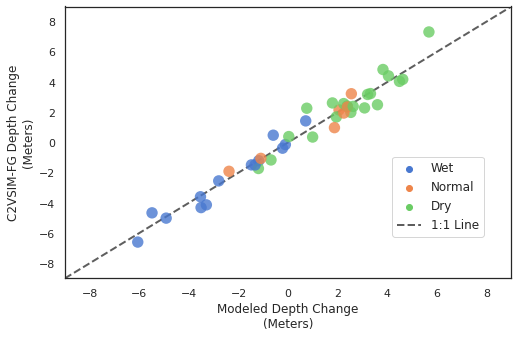
\includegraphics[width=0.6\textwidth]{results_gw_depth_response_calib.png}
    \caption{Results groundwater depth response function and C2VSIM-FG (\cite{dwr_c2vsimfg_2021}). Dots represent the median of each posterior predictive distribution of groundwater depth change, colors represent the water-year type in year t.}
    \label{fig:mesh1}
\end{figure}









\newpage
\printbibliography

\end{document}

